\chapter{Sistemi Complessi}
\section{Introduzione}
Verranno trattati degli stumenti per modellare e descrivere fenomeni naturali e reali
che variano nel tempo
\begin{definizione}[\textbf{Sistema complesso}]
    Un \textbf{Sistema complesso} è un insieme di unità semplici che cooperano tra
    di loro facendo emergere dei comportamenti complessi.
\end{definizione}
Verranno analizzati modelli discreti che sono facilmente implementabili utilizzati
nelle simulazioni, un sesempio sono:
\begin{itemize}
    \item \textbf{Automi cellulari}: paridigma di calcolo locale, parallelo e omogeneo
    \item \textbf{Subshift}: modelli per definire sistemi di condifica basata su
          parole proibite
    \item \textbf{Tiling}: modelli basati sul problema del tiling, ovvero ricoprire
          una superficie con delle piastrelle in modo tale che combaciano i colori sui
          lati di due piastrelle omogenee (problema NP-Hard).
\end{itemize}

Si studieranno le prorpietà dei fenomeni reali utilizzando i modelli e si mapperanno
le domande sulle proprietà dei modelli, in questo modo si potrà rispondere alle
domande analizzando le proprietà dei modelli.

\section{Automi cellulari (alfabeto finito)}
Gli automi cellulari sono delle reti di automi, gli automi, non per forza a stati
finiti, di cui sono composte possono essere uguali (automi cellulari uniformi) o differenti (automi cellulari non
uniformi). Lo stato dell'automa cellurare in un particolare momento dell'esecuzione
sarà l'insieme degli stati dei singoli automi nel particolare momento.

\begin{nota}
    Si parla di insieme degli stati del singolo automa perché può essere una
    sequenza nel caso di CA 1D, una matrice nel caso CA 2D, ecc$\dots$
\end{nota}

La transizione dell'automa cellulare dipende direttamente dalle transizioni dei singoli automi,
i quali, quando scattano, leggono il loro stato interno e gli stati degli automi
vicini e cambiano stato di conseguenza. Il cambio della configurazione dell'automa
cellulare coincide col cambiamento di stato di tutti gli automi della rete contemporaneamente.
Per questo gli automi cellulari sono un paradigma di calcolo:
\begin{itemize}
    \item locale
    \item parallelo
    \item uniforme (non uniforme)
\end{itemize}

\begin{nota}
    Gli automi cellulari sono dei paradigmi di calcolo universale perché si
    può convertire una qualsiasi Macchina di Turing in un automa cellulare
\end{nota}

\begin{nota}
    Gli automi cellulari sono delle reti di automi, un esempio di rete di automi
    è la rete neurale, in questo caso:
    \begin{itemize}
        \item non è uniforme perché ogni neurone può avere una funzione differente
        \item non è locale perché ogni neurone può non dipendere solo dai neuroni
              vicini
        \item è parallelo perché i neuroni scattano contemporaneamente
    \end{itemize}
\end{nota}

\begin{definizione} [\textbf{sequenze bi-infinite}]
    Dato un alfabeto $A$, chiameremo \textbf{sequenze bi-infinite} sull'alfabeto
    $A$ tutte quelle sequenze che sono infinite a destra ed infinite a sinistra.
\end{definizione}

\begin{esempio}
    Sia $A = \left\{0,1\right\}$ allora:
    \begin{itemize}
        \item $01101001110011$: è una sequenza finita
        \item $01101001110011\dots$: è una sequenza infinita a destra
        \item $\dots01101001110011$: è una sequenza infinita a sinistra
        \item $\dots01101001110011\dots$: è una sequenza bi-infinita
    \end{itemize}
\end{esempio}

\begin{definizione}[\textbf{spazio delle configurazioni}]
    Lo \textbf{spazio delle configurazioni} è
    $$A^\mathbb{Z}= \left\{x|x:\mathbb{Z}\rightarrow A\right\}$$
    Coincide con l'insieme di tutte le sequenze \textbf{bi-infinite} sull'alfabeto
    $A$
\end{definizione}
Lo spazio delle configurazioni è un insieme di funzioni, ciascuna funzione rappresenta
una sequenza \textbf{bi-infinita} che associa ad ogni indice in $\mathbb{Z}$ della
sequenza un carattere dell'alfabeto.
\begin{esempio}
    Sia $x\in A^\mathbb{Z}$, si può rappresentare nel sequente modo
    $$x = \left(\dots, x_{-2}, x_{-1},x_{0},x_{1},x_{2},\dots\right), \ \forall x_i\in A$$
    Con
    $$x(i) = x_i$$
\end{esempio}

Si studiano automi cellulari infiniti perché possono catturare tutti i comportamenti
del sistema, cosa che non posso fare con gli automi finiti. Essendo infiniti,
le singole configurazioni dell'automa devono essere infite, ecco perché si utilizzano
\textbf{sequenze bi-infinite}.

\begin{definizione} [\textbf{sottosequenza}]
    Possiamo definire le \textbf{sottosequenza} di una \textbf{sequenza bi-infinita}
    nel seguente modo.

    $\forall x \in A^{\mathbb{Z}}$ e $\forall h,k\in \mathbb{Z}$ con $h\le k$
    abbiramo:
    $$x_{[h,k]}= x_hx_{h+1}\dots x_k\in A^{k-h+1}$$
    La sottosequenza sarà finita e di lunghezza $k-h+1$.
\end{definizione}

Per studiare alcune proprietà degli automi cellulari si utilizzano i concetti di
distanza.
\begin{definizione}[\textbf{distanza su un generico insieme}]
    Dato un insieme $X$, una \textbf{funzione distanza} è una qualsiasi funzione
    $d:X\times X \rightarrow \mathbb{R}_+$ che soddisfa le sequenti proprietà:
    \begin{itemize}
        \item \textbf{non degenerazione}: $\forall x,y\in X, d(x,y) = 0\iff x=y$
        \item \textbf{simmetrica}: $\forall x,y\in X, d(x,y) = d(y,x)$
        \item \textbf{disuguaglianza triangolare}: $\forall x,y,z\in X, d(x,y) \le d(x,z)+d(z,y)$
    \end{itemize}
\end{definizione}

\begin{esempio}[distanza triviale]
    Un esempio di distanza è la seguente
    $$d(x,y) =\begin{cases}
            0 & x=y    \\
            1 & x\ne y \\
        \end{cases}$$
\end{esempio}

\begin{esempio}[distanza euclidea]
    Un esempio di distanza è la seguente
    $$d(x,y) =|x-y|$$
    Generalizzabile su $\mathbb{R}^n$ con la $|.|_2$$\dots$
\end{esempio}

A noi servirà una distanza tra le configurazioni di CA per poter confrontare
la vicinanza tra di loro e studiare le varie proprietà, utilizzeremo la distanza di
\textbf{Tychonoff}.
\begin{definizione} [\textbf{distanza su $A^\mathbb{Z}$}]
    $d:A^\mathbb{Z}\times A^\mathbb{Z} \rightarrow \mathbb{R}_+$ definita nel
    seguente modo:
    $$d(x,y) = \begin{cases}
            0             & x=y        \\
            \frac{1}{2^n} & altrimenti
        \end{cases}$$
    Dove $n= \min\left\{k\in \mathbb{N} | x_{[-k,k]} \ne y_{[-k,k]}\right\}$
\end{definizione}

La distanza si può anche non centrare nello $0$ ma in un altro indice differente,
ovviamente il calcolo cambia. Sia $d_i$ la distanza con il calcolo di $n$ centrato
in $i$ allora per ottenere $n$ si prende il valore $n'$ centrato in $i$ e si somma
l'offset dall'indice $0$.

\begin{nota} [Proprietà $1$ della distanza] \label{prop:dist}
    $\forall x,y\in A^\mathbb{Z}$, $\forall n\in \mathbb{N}$ vale che
    $$d(x,y)< \frac{1}{2^n}\iff x_{[-n, n]}=y_{[-n, n]}$$
\end{nota}

\begin{definizione}
    $(A^\mathbb{Z}, d)$ è lo \textbf{spazio metrico} delle configurazioni dell'automa
\end{definizione}

\begin{nota} [Proprietà $2$ della distanza]
    $(A^\mathbb{Z}, d)$ è un \textbf{spazio metrico compatto} cioè ogni successione
    di elementi di $A^\mathbb{Z}$ ammette una sottosuccessione convergente in $A^\mathbb{Z}$.
\end{nota}
\begin{definizione} [ \textbf{Automa cellulare 1D} ]
    Un \textbf{Automa cellulare 1D}  è una tripla $\langle A, r, f\rangle$
    dove:
    \begin{itemize}
        \item $A$: insieme finito di caratteri, corrisponde all'alfabeto dell'automa e
              quindi agli stati degli automi interni.
        \item $r\in \mathbb{N}$: raggio degli automi interni, specifica il raggio
              di dipendenza degli automi interni da quelli vicini. La transizione degli
              automi interni sarà dipendente dagli stati degli automi nel raggio
              di vicinanza $r$.
        \item $f: A^{2r+1}\rightarrow A$: regola locale di aggiornamento dello
              stato degli automi interni.
    \end{itemize}
\end{definizione}
Ad ogni $CA = \langle A, r, f\rangle$ viene associata una $F:A^\mathbb{Z}\rightarrow A^\mathbb{Z}$
chiamata \textbf{regola globale} che coincide con la specifica del cambiamento
di configurazione del $CA$.
\begin{definizione} [\textbf{Regola globale per CA}]
    $F:A^\mathbb{Z}\rightarrow A^\mathbb{Z}$, dati $\forall x \in A^\mathbb{Z}, i \in \mathbb{Z}$
    si definisce
    $$F(x)_i = f(x_{[i-r, i+r]})$$
    quindi
    \begin{table}[!h]
        \centering
        \begin{tabular}{ccccccccccc}
            $x$    & $=$ & $($ & $\dots$                     & $x_{i-r}$ & $\dots$                     & $x_i$ & $\dots$ & $x_{i+r}$ & $\dots$ & $)$ \\
            $F(x)$ & $=$ & $($ & \multicolumn{3}{c}{$\dots$} & $F(x)_i$  & \multicolumn{3}{c}{$\dots$} & $)$
        \end{tabular}
    \end{table}
\end{definizione}
\begin{definizione} [ \textbf{Automa cellulare 1D elementare} ]
    Gli \textbf{Automi cellulari 1D elementari} sono \textbf{Automi cellulari 1D}
    con $A=\{0,1\}$ e $r=1$
\end{definizione}

Più precisamente per rappresentare un CA  $\langle A, r, f\rangle$ ci sono 3 modi:
\begin{itemize}
    \item \textbf{tabella}: si scrive la tabella che definisce la regola locale
    \item \textbf{numero decimale}: si utilizza un numero decimale che condifica
          la regola locale, si può ricavare facilmente dalla tabella
          $$n_f = \{0,\dots, |A|^{|A|^{2r+1}-1}\}$$
    \item \textbf{grafo di De Bruijn}: si utilizza un grafo orientato
\end{itemize}


\begin{esempio} [Rappresentazione tabellare]
    Per rappresentare la regola locale in tabella, basta creare una tabella di
    $|A|^{2r+1}$ righe e $2$ colonne. Nella prima colonna si mettono per riga e in ordine
    tutte le combinazioni di input, nella seconda colonna si mette il carattere
    finale.
\end{esempio}

\begin{esempio} [Rappresentazione numero decimale]
    Per rappresentare la regola locale in numero decimale, basta rappresentare
    la regola locale in tabella e poi codificare in decimale il numero scritto in
    verticale dal basso verso l'alto nella seconda colonna. Ricorda che questo numero
    è in base $|A|$.
\end{esempio}

\begin{nota}
    Per gli CA elementari si ha che la regola locale è defina nel seguente modo
    $$f:\{0,1\}^3\rightarrow \{0,1\}$$
    Quindi si possono avere un totale di $256 = |\{0,1\}^3|
        = |C|^{|D|}$ regole locali che
    corrispondono quindi a $256$ CA 1D elementari e ogni automa è rappresentato da un
    numero $x\in [0, 255]$ che corrisponde alla conversione in decimale della regola
    locale.
\end{nota}

\begin{definizione} [\textbf{Grafo di De Bruijn}]
    Il \textbf{Grafo di De Bruijn} associato a CA $\langle A, r, f\rangle$ è $\langle V,E,l\rangle$
    dove:
    \begin{itemize}
        \item $V=A^{2r}$
        \item $E = \{(u,v)\in V\times V | u=u_1\dots u_{2r},  v=v_1\dots v_{2r} \text{ con } u_2\dots u_{2r} = v_1\dots v_{2r-1}\}$
        \item $l:E\rightarrow \{0,1\}$ funzione che etichetta gli archi nel seguente
              modo $$\forall (u,v)\in E, l(u,v) = f(u,v_{2r})=f(u_1,v)$$
    \end{itemize}
\end{definizione}

La rappresentazione a grafo è quella più riusabile perché se dovessimo cambiare
la regola locale allora basta solo aggiornare l'etichette degli archi. In aggiunta
data una regola locale generica $f$, possiamo risriverla nel segunete modo.
\begin{equation}
    f: A\times A^{2r} \rightarrow A \equiv \delta: Q\times \sigma \rightarrow Q
\end{equation}
Con $Q= A$ e $\sigma = A^{2r} $, così è possibile sottolineare la funzione di transizione
di ogni automa nel CA.
\subsection{ Mappa di Shift e teorema di Hedlund}
\begin{definizione} [\textbf{Mappa di shift}]
    La \textbf{mappa di shift} è la funzione $\sigma:A^\mathbb{Z}\rightarrow A^\mathbb{Z}$
    definita nel seguente modo
    $$\forall x\in A^\mathbb{Z}, \forall i \in Z, \sigma(x)_i=x_{i+1}$$
    \begin{table}[!h]
        \centering
        \begin{tabular}{ccccccccc}
            $x$         & $=$ & $($ & $\dots$ & $x_{i-1}$ & $x_i$     & $x_{i+1}$ & $\dots$ & $)$ \\
            $\sigma(x)$ & $=$ & $($ & $\dots$ & $x_{i}$   & $x_{i+1}$ & $x_{i+2}$ & $\dots$ & $)$
        \end{tabular}
    \end{table}
\end{definizione}

\begin{nota}
    La mappa di shift è la regola globale del CA $\langle A,r=1,f\rangle$ dove
    $f:A^3\rightarrow A$ è definita come $f(a,b,c) = c$. Con $|A|=2$ allora $f\equiv 170$

\end{nota}

\begin{teorema} [\textbf{Hedlund}] \label{th:hedlund}
    Sia $F:A^\mathbb{Z}\rightarrow A^\mathbb{Z}$ una qualunque funzione.
    $F$ è la regola globale di un CA \textbf{sse} entrambe le seguenti affermazioni
    sono vere:
    \begin{itemize}
        \item $F$ continua
        \item $F$ commuta con $\sigma$, ovvero $ F\circ\sigma =\sigma \circ F$
    \end{itemize}
    \begin{proof}
        Dimostriamo entrambe le implicazioni:
        \begin{itemize}
            \item $\implies$: partiamo col dimostrare che $F$ sia continua
                  $$\forall x \in A^\mathbb{Z}, \forall \epsilon > 0 \exists \delta> 0 \text{ t.c } \forall y \in A^\mathbb{Z}: d(y, x) < \delta \implies d(F(y), F(x))< \epsilon$$
                  Bene, scegliamo arbitrariamente $x\in  A^\mathbb{Z}$ e $\epsilon >0$.
                  Sia $n\in \mathbb{N}$ tale che $\frac{1}{2^n} < \epsilon $, facciamo vedere
                  che $\exists \delta>0$ tale che
                  $$\forall y\in A^\mathbb{Z}, d(y,x) < \delta \implies d(F(y), F(x))< \frac{1}{2^n}$$
                  con $\delta=\frac{1}{2^{n+r}}$ è vera. Perché per la prima proprietà
                  della distanza e per la sua definizione (vedi nota \ref{prop:dist}) abbiamo che $d(F(y),F(x)) < \frac{1}{2^{n}}$
                  quindi significa che $F(x)_{[-n,n]} = F(y)_{[-n,n]}$ quindi per
                  $\delta=\frac{1}{2^{n+r}}$ è vero che $d(y,x) < \frac{1}{2^{n+r}}$
                  che significa sempre per la stessa proprietà che $x_{[-n-r,n+r]} = y_{[-n-r,n+r]}$.
                  Tutto viene spiegato dal fatto che se non fossero uguali le sottosequenze
                  di $x$ e $y$ allora non possono essere uguali le sottosequenze di $F(x), F(y)$.
                  Abbiamo dimostrato la continuità.

                  Successivamente dimostriamo $F\circ \sigma = \sigma \circ F\implies F(\sigma(x)) = \sigma(F(x)), \forall x \in A^\mathbb{Z}$.
                  l'uguaglianza precedente può essere riscritta come $\forall x \in A^\mathbb{Z}, \forall i \in \mathbb{Z}, (F(\sigma(x)))_i =(\sigma(F(x)))_i$.
                  Possiamo notare che
                  $$(F(\sigma(x)))_i = f(\sigma(x)_{[i-r,i+r]})=f(x_{[i-r+1,i+r+1]})$$
                  Inoltre
                  $$(\sigma(F(x)))_i =F(x)_{i+1} =f(x)_{[i+1-r,i+1+r]}$$
                  Abbiamo dimostrato che commutano.
            \item $\impliedby$: dobbiamo dimostrare che esiste la tripla che definisce il CA.
                  Per prima cosa conosciamo l'alfabeto che è $A$ ricavato da $F$. Successivamente
                  datto che $F$ è continua e $A^\mathbb{Z}$ è compatto allora $F$ è \textbf{uniformemente
                      continua}, ossia $\forall\epsilon >0,\exists \delta > 0 \text{ t.c. } \forall x,y \in A^\mathbb{Z}$
                  abbiamo $d(y,x)<\delta \implies d(F(y), F(x)) < \epsilon$. Scegliamo $\epsilon = 1\implies \frac{1}{2^0}\implies n=0\implies F(y)_0= F(x)_0$
                  sicuramente sappiamo che $\exists \delta >0$ tale che $$\forall x,y \in A^\mathbb{Z} d(y,x)<\delta \implies d(F(y), F(x)) < 1$$
                  Ovvero $$\forall x,y \in A^\mathbb{Z} d(y,x)<\delta \implies F(y)_0= F(x)_0$$
                  Sia $r\in \mathbb{N}$ il più piccolo numero t.c. $\frac{1}{2^r}<\delta$.
                  Allora $\forall x,y \in A^\mathbb{Z}$
                  $$d(y,x)<\frac{1}{2^r} \implies F(y)_0= F(x)_0$$
                  Ovvero $\forall x,y \in A^\mathbb{Z}$
                  $$y_{[-r,r]} =x_{[-r,r]}\implies F(y)_0= F(x)_0$$
                  Quindi abbiamo trovato $r$.

                  Facciamo vedere che $F$ sia la regola globale, ovvero determiniamo $f$, cioè
                  $\forall x\in A^\mathbb{Z},\forall i\in\mathbb{Z}$
                  $$F(x)_i = f(x_{[i-r,i+r]})$$
                  Sia $f: A^{2r+1}\rightarrow A$ definita come $\forall u \in A^{2r+1}$
                  $$f(u) = F(z)_0$$ dove $z$ è una qualunque configurazione di
                  $A^\mathbb{Z}$ tale che $z_{[-r,r]} = u$. Bisogna però controllare che
                  la definizione sia ben posta per ogni valore $z$. Lo è dal momento che
                  $\forall z',z''\in A^\mathbb{Z}: z'_{[-r,r]} =  z''_{[-r,r]}\implies F(z')_0 = F(z'')_0$.
                  Ora mostriamo che sia vera $\forall x\in A^\mathbb{Z}$
                  $$F(x)_i = f(x_{[i-r,i+r]}) = 0$$
                  Questo è vero perché discende dalla definizione di $f$ con $z = x$.
                  Ora mostriamo che sia vera $\forall x\in A^\mathbb{Z}$
                  $$F(x)_i = f(x_{[i-r,i+r]})\ne 0$$
                  $$F(x)_i = (\sigma^i(F(x)))_0=(F(\sigma^i(x)))_0=f(\sigma^i(x)_{[-r,r]}) = f(x_{[i-r,i+r]}) \ne 0$$
        \end{itemize}
    \end{proof}
\end{teorema}

\begin{definizione}
    Un elemento $x\in A^\mathbb{Z}$ è detto \textbf{configurazione spazialmente
        periodica} sse $\exists k>0 $ t.c. $\sigma^k(x) = x$, o equivalentemente, sse
    $\exists u\in A^k$ con $k>0, x = ^\infty u ^\infty$. Cioè $x$ è una ripetizione
    bi-infinita di $u$.
\end{definizione}

Il teorema \ref{th:hedlund} ha le seguenti conseguenze conseguenze:
\begin{itemize}
    \item se $x\in A^\mathbb{Z}$ è \textbf{spazialmente periodica} allora $y=F(x)$
          è  \textbf{spazialmente periodica}
          \begin{proof}
              Se $x\in A^\mathbb{Z}$  è spazialmente periodica $\implies\exists k>0$ t.c.
              $\sigma^k(x)=x \implies F(\sigma^k(x)) = F(x)\implies \sigma^k(F(x))$.
              Si noti che se $x$ è la ripetizione di una parola di lunghezza $k>0$ allora
              anche $F(x)$ è la ripetizione di una parola di lunghezza $k$. Perciò dopo
              un numero finito di applicazioni consecutive di $F$ (al più $k$), si riuscirà
              a riottenere la stringa già ottenuta dalle applicazioni precedenti dal momento
              che si effettua una permutazione di una stringa $k$. Infatti l'\textbf{evoluzione
                  periodica} poiché $A^k$ è un insieme finito.
          \end{proof}
    \item Dato un $CA = <A,r,f>$ con regola globale $F$, è possibile definire un  $CA '= <A,2r,f'>$
          con regola globale $F'$ tale che $F'=F^2$ con $f'$ definita in questo modo.
          $$f':A^{4r+1}\rightarrow A$$
          Dove $\forall u=u_1\cdots u_{4r+1}\in A^{4r+1}$
          $$f'(u) = f'(f(u_1\cdots u_{2r+1})f(u_{2}\cdots u_{2r+2})\cdots f(u_{2r+1}\cdots u_{4r+1}))$$
          Per dimostrare che $F^2$ sia una regola globale possiamo utilizzare il teorema di
          hedlund:
          \begin{itemize}
              \item \textbf{continuità}: si perché $F^2$ è una composizione di funzioni $F$ 
              che sono continua
              \item \textbf{commutatività}: $F^2\circ \sigma = F\circ (F\circ \sigma ) = F\circ (\sigma\circ F  ) = \sigma\circ (F\circ F  )  = \sigma \circ F^2$
          \end{itemize}
          Quindi è una regola globale.
    \item Siano $F$ e $G$ due regole globali di due $CA$ differenti sullo stesso
          alfabeto $A$. $F\circ G$ è una regola globale di un CA? Possiamo dimostrarlo con
          il teorema:
          \begin{itemize}
              \item \textbf{continuità}: si perché è una composizione di funzioni continue
              \item \textbf{commutatività}: $F\circ (G\circ \sigma) = F\circ (\sigma\circ G) = (F\circ \sigma)\circ G =(\sigma\circ F)\circ G = \sigma\circ (F\circ G)$
          \end{itemize}
    \item Sia $F$ la regola globale per CA, supponiamo che $F$ sia invertibile,
          allora $F^{-1}$ è una regola globale per CA? Dimostriamolo:
          \begin{itemize}
              \item \textbf{continuità}: si perché $A^\mathbb{Z}$ è compatto
              \item \textbf{commutatività}: $$F\circ \sigma = \sigma \circ F $$
                    $$ F^{-1} \circ F\circ \sigma \circ F^{-1}= F^{-1}\circ \sigma \circ F \circ F^{-1}$$
                    $$ (F^{-1} \circ F)\circ \sigma \circ F^{-1}= F^{-1}\circ \sigma \circ (F \circ F^{-1})$$
                    $$ \sigma \circ F^{-1}= F^{-1}\circ \sigma$$
          \end{itemize}
\end{itemize}

\subsection{Iniettività e suriettività degli automi cellulari}

\begin{definizione} [\textbf{Estensione della regola locale}]
    L'\textbf{estensione della regola locale} per parole di lunghezza maggiore di
    $2r+1$. coincide con la regola globale ma
    applicata ad una stringa finita. Formalmente, $f^\ast: A^\ast\rightarrow A^\ast$
    tale che $\forall u\in A^\ast$:
    \begin{equation*}
        f^\ast(u) = \begin{cases}
            \epsilon                                                             & |u| < 2r+1 \\
            f(u_1\dots u_{2r+1})f(u_2\dots u_{2r+2})\dots f(u_{n-2r}\dots u_{n}) & altrimenti
        \end{cases}
    \end{equation*}
\end{definizione}

\begin{nota}
    Se $A^\ast\equiv A^\mathbb{Z}\implies F \equiv f^\ast$.
\end{nota}

\begin{nota}
    Per la suriettività di $F$ sarà importante conoscere se $f$ è bilanciata ovvero
    se $|f^{-1}(0)| =|f^{-1}(1)|$, dove $  f^{-1}(y)$ coincide con l'insieme delle
    preimmagini di $y$.
\end{nota}

\begin{nota}
    Sia un CA $\langle A,r,f\rangle$ e $G$ il suo grafo di De Bruijn associato.
    I cammini bi-infiniti sui vertici di $G$ sono in corrispondenza biunivoca
    con gli elementi di $A^\mathbb{Z}$. Inoltre, $\forall x\in A^\mathbb{Z}$ ($ \forall u\in A^\ast$)
    $F(x)$ ($f^\ast(u)$) è dato dalle etichette degli archi del cammino sui vertici
    corrispondente a $x$ ($u$).
    \begin{proof}
        Deriva dalla definizione del grafo di De Bruijn associato ad un automa cellulare.
    \end{proof}
\end{nota}

Questo è vero perché due nodi consecutivi in un cammino corrispondono ad un elemento
del dominio di $f$, mentre l'etichetta dell'arco corrisponde all'immagine dell'elemento
stesso.

\begin{nota}
    Il grafo di De Bruijn $G$ di un CA $\langle A,r,f\rangle$ può essere considerato
    come un \textbf{automa a stati finiti non deterministico} in cui tutti i nodi sono sia stati iniziali, sia
    stati finali. Questi particolari automi sono chiamati \textbf{automi di Fisher}
\end{nota}

Questi automi sono importanti perché permettono di accettare il linguaggio composto
da parole bi-infinite che rappresentano tutte le possibili configurazioni dell'automa
cellulare, sia bi-infinite, sia parziali.

Da notare che dal grafo di De Bruijn otteniamo degli automi non deterministici,
per la teoria degli automi possiamo facilmente ricavare l'automa deterministico
calcolando l'insieme potenza degli stati.

\begin{definizione} [\textbf{Suriettività}]
    La definizione di \textbf{suriettività} di un automa cellulare è quando la sua
    \textbf{regola globale} è \textbf{suriettiva} ovvero:
    \begin{itemize}
        \item $\forall y\in A^\mathbb{Z},\exists x\in A^\mathbb{Z}: F(x) = y$
        \item $F(A^\mathbb{Z}) = A^\mathbb{Z}$
        \item $\forall y \in A^\mathbb{Z}, F^{-1}(y) \ne \emptyset $
    \end{itemize}
    Dove $F^{-1}(y)$ è l'insieme delle preimmagini di $y$.
\end{definizione}

La suriettività è una proprietà di \textbf{raggiungibilità debole}

\begin{nota}
    Il significato di $f^{\ast}$ bilanciato significa che $\forall n\in \mathbb{N}, n>0$
    ogni parola di $u\in A^n$ ha lo stesso numero di preimmagini. Questo significa
    chiedere che ogni parola del dominio di $f^{\ast}$ ($|A|^{n+2r}$) abbia lo stesso
    numero di immagini ($|A|^n$). Questo significa che il numero di preimmagini
    sarà
    \begin{equation*}
        |A|^{2r} = \frac{|A|^{n+2r}}{|A|^n} = \frac{|Dom|}{|CoDom|}
    \end{equation*}
\end{nota}

\begin{teorema}
    \label{th:suriettività_CA}
    Sia $\langle A,r,f\rangle$ un CA e sia $F: A^\mathbb{Z}\rightarrow A^\mathbb{Z}$
    la regola globale. Sia $G$ il grafo di De Bruijn associato all'automa cellulare.
    Sia $\mathcal{L}$ il linguaggio associato all'automa ottenuto dal grafo di De Bruijn.
    Allora le seguenti affermazioni sono equivalentementi:
    \begin{enumerate}
        \item \label{cond:1}$F$ è \textbf{suriettiva}
        \item \label{cond:2}$f^\ast$ è \textbf{bilanciata} ossia $\forall u \in A^+ (u\ne \epsilon), |f^{\ast^{-1}}(u)|= |A^{2r}|$
        \item \label{cond:3}$\mathcal{L} = A^\ast$
    \end{enumerate}
    \begin{proof}
        Dimostriamo le singole implicazioni:
        \begin{itemize}
            \item $\ref{cond:1}\implies \ref{cond:2}$: la dimostrazione si basa
                  sul dimostrare $\lnot \ref{cond:2}\implies \lnot \ref{cond:1}$.

                  Ipotizziamo per assurdo che $\exists u\in A^n$ t.c. $|f^{\ast^{-1}}(u)|\ne |A|^{2r}$.
                  Senza perdere di generalità assumiamo che $|f^{\ast^{-1}}(u)|< |A|^{2r}$,
                  non perdiamo generalità perché se prendessimo $u$ tale che $|f^{\ast^{-1}}(u)|> |A|^{2r}$
                  allora esisterà un'altra stringa $u'$ tale che $|f^{\ast^{-1}}(u')|< |A|^{2r}$,
                  in caso avremmo preso quella.

                  Sia $s = |f^{\ast^{-1}}(u)|$, sia $k>1$ un numero arbitrario allora costruiamo
                  i seguenti insiemi di parole:
                  \begin{itemize}
                      \item $V$: sarà la giustapposizione di $k$ preimmagini qualunque
                            di $u$. Quindi $|V| = s^k$
                      \item $W$: contenente parole del tipo $w=(uA^{2r})^{k-1}u$. Quindi $|W| = |A|^{(k-1)2r}$
                  \end{itemize}

                  Per costruzione sappiamo che $\forall v\in V, f^{\ast}(v)\in W$, ma $\exists
                      w'\in W\text{ t.c. } f^{\ast^{-1}} (w')= \emptyset$? (si sta controllando se non è suriettiva)

                  Sicuramente $w'$ esiste se $|V|<|W|$, ovvero  $s^k<(|A|^{2r})^{(k-1)}$.
                  Sapendo che $s^k < |A|^{2r}$ allora $\exists k$ tale che  $|V|<|W|$.
                  Quindi $\exists w \in W: f^{\ast^{-1}} (w) =\emptyset$, perciò
                  $\exists y \in A^{\mathbb{Z}}: F^{-1}(y) = \emptyset$, basta scegliere
                  $y$ che contiene $w$. Concludiamo che $F$ non è surettiva.

            \item $\ref{cond:2}\implies \ref{cond:3}$: occorre mostrare che $\mathcal{L} \subseteq A^\ast$
                  e allo stesso tempo $ A^\ast \subseteq\mathcal{L}$. La prima deriva
                  dalla definizione di $\mathcal{L}$, quindi ci basta dimostrare
                  $A^\ast \subseteq\mathcal{L}$. Scegliamo arbitrariamente $v\in  A^\ast$,
                  mostriamo che $v\in \mathcal{L}$, ossia che $v$ si ottiene dalla concatenazione
                  delle etichette degli archi di un cammino sui vertici di $v$.

                  Siccome $|f^{\ast^{-1}}(v)| = |A|^{2r}$, in particolare $\exists u \in A^\ast$
                  t.c $f^\ast(u) = v$. Per definizione di $G$, siccome $u$ corrisponde
                  ad un cammino finito sui vertici di $G$, $f^\ast(u)=v$ si ottiene dalle etichette
                  degli archi di quel cammino.
            \item $\ref{cond:3}\implies \ref{cond:1}$: scelto arbitrariamente $y\in A^\mathbb{Z}$,
                  occorre mostrare che $\exists x\in A^\mathbb{Z} \text{ t.c. } F(x) =y$.

                  Sia $y\in A^\mathbb{Z}$ scelto arbitrariamente. $\forall n\in \mathbb{N}$
                  sia $v^{(n)} = y_{[-n,n]}\in A^{2n+1}$.

                  Per ipotesi sappiamo $\exists u^{(n)}\in f^{\ast^{-1}}(v^{(n)})\subseteq A^{2n+2r+1}$.
                  Quindi $f^{\ast^{-1}}(u^{(n)}) = v^{(n)}$.

                  Sia $x^{(n)}\in A^\mathbb{Z}$ una qualunque configurazione tale che
                  $$x^{(n)}_{[-n-r,n+r]} = u^{(n)}$$

                  Non è detto che $F(x^{(n)})=y$, vale sicuramente che $\forall n \in \mathbb{N},F(x^{(n)})_{[-n,n]}=y_{[-n,n]}$,
                  ossia che $d(F(x^{(n)})_{[-n,n]},y_{[-n,n]})< \frac{1}{2^n}$.

                  Inoltre, $\{x^{(n)}\}_{n\in \mathbb{N}}$ ammette una sottosuccessione
                  $\{x^{(n_h)}\}_{h\in \mathbb{N}}$ convergente (per la compattezza di $A^{\mathbb{N}}$).
                  Ovvero sia $x= \lim\limits_{h\rightarrow +\infty}x ^{(n_h)}$ otteniamo  che $$ F(x)= F(\lim\limits_{h\rightarrow +\infty}x ^{(n_h)}) = \lim\limits_{h\rightarrow +\infty} F(x^{(n_h)})=y$$,
                  quindi $\exists x \in A^\mathbb{Z}$ t.c. $y = F(x)$
        \end{itemize}
    \end{proof}
\end{teorema}

\begin{teorema}
    La suriettività è una proprietà decidibile per un CA \textbf{monodimensionale}.
    \begin{proof}
        Basta dimostrare la condizione \ref{cond:3} del teorema \ref{th:suriettività_CA}
        che è decidibile. I passi per dimostrarlo sono i seguenti:
        \begin{itemize}
            \item Si costruisce l'automa di Fisher dall'automa di De Bruijn associato al CA
            \item Trasformo l'automa in deterministico
            \item Minimizzo l'automa
            \item Controllo se il linguaggio accettato dall'automa minimizzato $\mathcal{L}$ sia
                  uguale a $A^\ast$. Per farlo controllo che da ogni stato posso leggere
                  tutti i caratteri di $A$.
        \end{itemize}
    \end{proof}
\end{teorema}
\begin{nota}
    Per controllare se $\mathcal{L} = A^\ast$ occorre costruire l'automa deterministico
    che risconosce $ \mathcal{L}$. Tale automa ha $\mathcal{P}(V)$ come insieme di
    vertici e quindi significa che la complessità dell'algoritmo decibile è maggiore
    di $|\mathcal{P}(V)| = 2^{|A|^{2r}}$. Con questo approccio non possiamo ridurre
    la complessità perché è vincolata dai nodi del grafo di De Bruijn.
\end{nota}

\begin{nota}
    La suriettività è indecidibile da dimostrare utilizzando la condizione \ref{cond:2}
    del teorema \ref{th:suriettività_CA} perché dobbiamo controllare $\forall u \in A^+$ (indecidibile),
    questo significa che questa condizione è più utile per dimostrare la \textbf{non
        suriettività}, dal momento che ce ne basta una sola (semidecidibile).
\end{nota}

\begin{definizione}[\textbf{configurazione $q$-finita}]
    Sia $q\in A$, $x\in A^\mathbb{Z}$ è una \textbf{configurazione $q$-finita}
    se $|\{i\in \mathbb{Z}| x_i\ne q\}|< \infty$ ossia se $x$ è della forma:
    \begin{table}[!h]
        \centering
        \begin{tabular}{ccccccccc}
            $x$ & $=$ & $($ & $\dots$ & $qqqqq$ & $u$ & $qqqqq$ & $\dots$ & $)$ \\
        \end{tabular}
    \end{table}
    per qualsiasi $u\in A^\ast$
\end{definizione}

\begin{definizione}
    Definiremo:
    \begin{itemize}
        \item $\mathcal{F}$: l'insieme delle \textbf{configurazioni $q$-finite}
        \item $\mathcal{SP}$: l'insieme delle \textbf{configurazioni spazialmente periodiche}
              \begin{equation*}
                  \mathcal{SP}= \{x\in A^\mathbb{Z} | \exists k \in \mathbb{N}, k>0 \text{ t.c. }\sigma^k(x)=x\}
              \end{equation*}
    \end{itemize}
\end{definizione}

\begin{teorema}
    Sia $\langle A,r,f\rangle$ un CA allora le seguenti affermazioni sono equivalentementi:
    \begin{enumerate}
        \item $F$ è \textbf{suriettiva}
        \item $F_{\mathcal{SP}}$ è \textbf{suriettiva} (ovvero $F$ ristretta a $\mathcal{SP}$ è suriettiva)
        \item $\forall x,y \in \mathcal{F}, x\ne y \implies F(x)\ne F(y)$ (ovvero $F$ iniettiva sulle \textbf{configurazioni $q$-finite})
    \end{enumerate}
\end{teorema}

\begin{teorema}
    Se $F$ è iniettiva allora $F$ è iniettiva sulle spazialmente periodiche quindi
    $F$ è anche suriettiva.
\end{teorema}

\begin{teorema}
    \label{th:iniettiva}
    Sia $\langle A,r,f\rangle$ un CA allora le seguenti affermazioni sono equivalentementi:
    \begin{enumerate}
        \item $F$ è \textbf{iniettiva}
        \item $\exists m \le |A|^{4r} \textbf{ t.c. } \forall x, y \in A^\mathbb{Z} F(x)_{[-m,m]}=F(y)_{[-m,m]} \implies x_0=y_0$
              (caso bi-infinito)
        \item \label{cond:th_ini_3}$\exists m \le |A|^{4r} \textbf{ t.c. } \forall u,v \in A^{2m+2r+1} f(u)= f(v) \implies u_{m+r+1} = v_{m+r+1}$
              (caso finito)
    \end{enumerate}
\end{teorema}
\begin{teorema}
    L'iniettività è una proprietà decidibile per gli CA unidimensionali

\end{teorema}
La proprietà \ref{cond:th_ini_3} del teorema \ref{th:iniettiva} è decidibile perché
abbiamo anche un algoritmo per risolvere il problema (vedi figura \ref{fig:algo_iniettiva}).
\begin{figure}[!h]
    \centering
    \includegraphics[width=.7\textwidth]{img/sistemi_complessi/algoritmo_iniettività.png}
    \caption{Pseudocodice dell'algoritmo per testare la condizione \ref{cond:th_ini_3} del teorema \ref{th:iniettiva}}
    \label{fig:algo_iniettiva}
\end{figure}
\begin{nota}
    La complessità dell'algoritmo è maggiore di circa
    \begin{equation*}
        \frac{1}{2} \sum_{m=0}^{|A|^{4r}} |A|^{2(2m+2r+1)} = \frac{1}{2}  |A|^{4r+2}
        \frac{1-(|A|^4)^{|A|^{4r}+1}}{1-|A|^4}
    \end{equation*}
\end{nota}

Quindi per gli CA le seguenti proprità sono equivalenti:
\begin{itemize}
    \item iniettività
    \item suriettività (esiste la regola globale inversa)
    \item reversibilità
\end{itemize}

\begin{teorema}
    $F$ è iniettiva $\iff$ $F_{\mathcal{SP}}$ è iniettiva
\end{teorema}

\begin{teorema}
    $F$ non è suriettiva $\iff$ $\exists$ un \textbf{diamente}, cioè se
    $\exists w \in A^{2r}, \exists u,v \in A^+, u\ne v$ con $|u|=|v|$ t.c. $f(wuw)=f(wvw)$
    \begin{proof}
        La dimostrazione dell'$\impliedby$ viene fatta costruendo $w^\infty u w^\infty$
        e $w^\infty v w^\infty$ e controllando che $F(w^\infty u w^\infty) = F(w^\infty v w^\infty)$
        in modo da trovare la non inettività e quindi la non suriettività.
    \end{proof}
\end{teorema}

\begin{definizione}[\textbf{Grafo automa prodotto}]
    Sia $G=(V,E,l)$ un grafo di De Bruijn di un CA, il \textbf{Grafo prodotto}
    è $(V\times V,E',l')$ dove $$e'=((u',v'), (u'',v''))\in E'\land l(u',v') = l(u'',v'') = l'(e')$$
\end{definizione}

Sapendo che un cammino sul De Bruijn corrisponde all'immagine della configurazione
parziale o bi-infinita dell'automa, il cammino sul grafo prodotto corrisponde
a $2$ configurazioni dell'automa che condividono la stessa immagine. Quindi
formalmente un cammino bi-infinito sul grafo prodotto corrisponde ad una coppia
$(x',x'')\in A^\mathbb{Z} \times A^\mathbb{Z} $ tale che $F(x')=F(x'')$.

\begin{definizione}[\textbf{Diagonale del grafo prodotto}]
    Dato un grafo prodotto $(V\times V,E',l')$ allora la \textbf{Diagonale del grafo prodotto}
    $\Delta$ è definita nel seguente modo
    $$\Delta = \{(u,u)| u \in V\}\subseteq V\times V$$
\end{definizione}
La diagonale corrisponde ad un isomorfismo del grafo di De Bruijn e un cammino
bi-infinito sulla diagonale corrisponde ad un cammino bi-infinito sul grafo di De
Bruijn (vedi figura \ref{fig:automa_prodotto}).

\begin{figure}[!h]
    \centering
    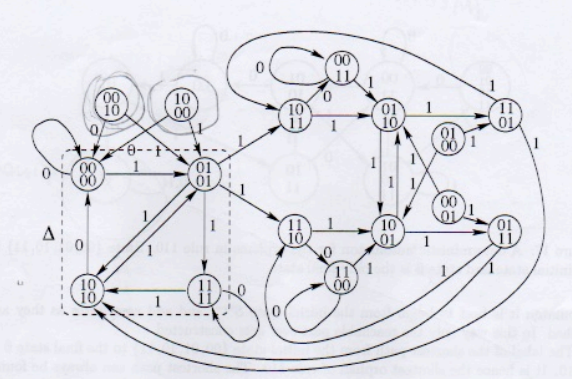
\includegraphics[width=.7\textwidth]{img/sistemi_complessi/automa_prodotto.png}
    \caption{Esempio di automa prodotto con la sua diagonale}
    \label{fig:automa_prodotto}
\end{figure}

\begin{teorema}
    Dato un automa CA monodimensionale allora \textbf{non è iniettivo} sse:
    \begin{enumerate}
        \item \label{cond:non_iniettiva_1} il suo grafo prodotto ha un ciclo che contiene un nodo fuori $\Delta$
        \item \label{cond:non_iniettiva_2}il suo grafo prodotto ha un ciclo che contiene un nodo in $\Delta$ e
              un nodo fuori $\Delta$
    \end{enumerate}
    \begin{proof}
        Dimostriamo i singoli punti:
        \begin{itemize}
            \item condizione \ref{cond:non_iniettiva_1}: se CA non è iniettivo
                  allora non è iniettivo sulle spazialmente periodiche. Quindi esisteranno
                  due configurazioni $c,e, c\ne e$ spazialmente periodiche tali che $F(c) = F(e)$,
                  quindi esisterà un camino sul grafo prodotto composto dai vertici che
                  rappresentano $c$ ed $e$. Il precedente cammino sarà composto da un ciclo
                  contenente nodi fuori dalla diagonale dal momento che $c\ne e$ per la
                  definizione di diagonale. Viceversa, dato un ciclo sul grafo prodotto contenente nodi
                  fuori dalla diagonale, allo questo significa che rappresenta due
                  configurazioni differenti aventi la stessa immagine, quindi CA non è
                  iniettivo.
            \item condizione \ref{cond:non_iniettiva_2}: Sia $q\in A$ arbitrario.
                  Se CA non è suriettivo allora significa che non è iniettivo sulle
                  configurazioni $q$-finite. Quindi esistono $c,e$ con $c\ne e $ configurazioni
                  $q$-finite tali che $F(c) =F(e)$. Il cammino corrispondente sul
                  grafo prodotto sarà composto da un ciclo all'interno di $\Delta$
                  seguito da un ciclo che esce da $\Delta$ per poi ritornare in $\Delta$.
                  Questo significa che il ciclo è composto da nodi sia nella diagonale,
                  sia fuori; quindi non è iniettivo. Viceversa, dato un ciclo composto da nodi nella diagonale
                  e fuori dalla diagonale, allora si ha un diamente, quindi CA non è suriettivo.

        \end{itemize}
    \end{proof}
\end{teorema}
Il grafo prodotto può essere ridotto rimuovendo alcune informazioni (figura \ref{fig:automa_prodotto_ridotto}):
\begin{itemize}
    \item tutti i nodi $v',v'' \in V\times V$ tali che $v'= (u,u'), v''=(u',u)$
          allora rappresentano le stesse configurazioni specchiate, quindi possono essere
          accorpati
    \item la diagonale può essere ridotta ad un unico nodo
\end{itemize}

\begin{figure}[!h]
    \centering
    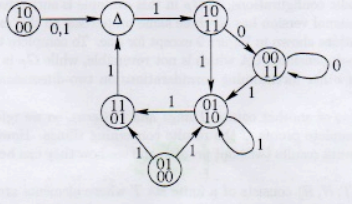
\includegraphics[width=.7\textwidth]{img/sistemi_complessi/automa_prodotto_ridotto.png}
    \caption{Esempio di automa prodotto ridotto}
    \label{fig:automa_prodotto_ridotto}
\end{figure}

Per scoprire se in un grafo ci sono dei cicli basta effettuare una DFS che ha una
complessità di $\mathcal{O}(|V|+|E|)$ e sapendo che $|V|= |V|^2$ dell'automa di
De Bruijn allora abbiamo un algoritmo polinomiale che ci permette di decidere
se il CA è suriettivo o iniettivo oppure no.

\subsection{Stabilità ed instabilità degli automi cellulari}
La notazione che verrà introdotto è valida per un qualsiasi \textbf{sistema dinamico a tempo
    discreto} (DTDS), ovvero per ogni $(X,F)$ dove $(X,d)$ è uno spazio metrico e
$F:X\rightarrow X$ è una trasformazione continua. Nel nostro caso $X \equiv A^\mathbb{Z}$,
$F$ è la regola globale e $d$ è la distanza di Tychonoff.

\begin{definizione} [\textbf{Punto di stabilità (equicontinuo, Lyapunov stable)}]
    % TODO: controllare not equal se va solo nelle definizioni di instabilità o anche in quelle di stabilità
    $x\in X$ è un \textbf{punto stabile} (equicontinuo, Lyapunov stable) sse
    $$\forall \epsilon > 0,\exists \delta > 0, \forall y\in X, d(y,x) < \delta \implies \forall t\in \mathbb{N} d(F^t(y),F^t(x))< \epsilon$$

    Con $X \equiv A^\mathbb{Z}$ e $d$ distanza di Tychonoff allora possiamo riscrivere
    la definizione in questo modo, $x\in X$ è un \textbf{punto stabile} sse
    $$\forall n\in \mathbb{N} ,\exists m\in \mathbb{N} , \forall y\in A^\mathbb{Z}, d(y,x) < \frac{1}{2^m} \implies \forall t\in \mathbb{N} d(F^t(y),F^t(x))< \frac{1}{2^n}$$
    Equivale a dire:
    $$\forall n\in \mathbb{N} ,\exists m\in \mathbb{N} , \forall y\in A^\mathbb{Z}, y_{[-m,m]} = x_{[-m,m]} \implies \forall t\in \mathbb{N} F^t(y)_{[-n,n]}=F^t(x)_{[-n,n]}$$

\end{definizione}
Questa coincide con la definizione di continuità con l'aggiunta del controllo che
sia continua anche sulle successive applicazioni, quindi per i successivi passi
temporali.

\begin{definizione} [\textbf{Punto di instabilità}]
    $x\in X$ è un \textbf{punto instabile} sse $x$ \textbf{non è stabile}

    $$\exists \epsilon > 0,\forall \delta > 0, \exists y\in X,x \ne y, d(y,x) < \delta \land \exists t\in \mathbb{N} d(F^t(y),F^t(x))\ge \epsilon$$

    Con $X \equiv A^\mathbb{Z}$ e $d$ distanza di Tychonoff allora possiamo riscrivere
    la definizione in questo modo,
    $$\exists n\in \mathbb{N} ,\forall m\in \mathbb{N} , \exists y\in A^\mathbb{Z},x \ne y, d(y,x) < \frac{1}{2^m} \land \exists t\in \mathbb{N} d(F^t(y),F^t(x))\ge \frac{1}{2^n}$$
    Equivale a dire:
    $$\exists n\in \mathbb{N} ,\forall m\in \mathbb{N} , \exists y\in A^\mathbb{Z},x \ne y, y_{[-m,m]} = x_{[-m,m]} \land \exists t\in \mathbb{N} F^t(y)_{[-n,n]}\ne F^t(x)_{[-n,n]}$$

\end{definizione}

\begin{definizione} [\textbf{Sistema stabile (stabilità globale)}]
    $(X,F)$ è \textbf{stabile} se $\forall x \in X$, $x$ è un \textbf{punto stabile}
\end{definizione}

\begin{definizione} [\textbf{Sistema equicontinuo (equicontinuità)}]
    $(X,F)$ è \textbf{equicontinuo} dove la definizione di stabilità di un punto cambia
    perché $\epsilon$ non dipende per un particolare punto $x\in X$ ovvero
    $$\forall \epsilon > 0,\exists \delta > 0, \forall y, x\in X, d(y,x) < \delta \implies \forall t\in \mathbb{N} d(F^t(y),F^t(x))< \epsilon$$
\end{definizione}

\begin{nota}
    L'equicontinuità è più stringente rispetto alla stabilità globale. Quando $X=A^\mathbb{Z}$
    si hanno due definizioni equivalenti e possono essere riscritte come
    $$\forall n\in \mathbb{N} ,\exists m\in \mathbb{N} , \forall y,x\in A^\mathbb{Z}, y_{[-m,m]} = x_{[-m,m]} \implies \forall t\in \mathbb{N} F^t(y)_{[-m,m]}=F^t(x)_{[-n,n]}$$
\end{nota}
\begin{definizione} [\textbf{Sistema instabile (instabilità globale)}]
    $(X,F)$ è \textbf{instabile} se $\forall x \in X$, $x$ è un \textbf{punto instabile}
\end{definizione}

\begin{definizione} [\textbf{Sistema sensibile alle condizioni iniziali (effetto butterfly)}]
    $(X,F)$ è \textbf{sensibile alle condizioni iniziali} se
    $$\exists \epsilon > 0,\forall x \in X, \forall \delta > 0, \exists y\in X,x \ne y, d(y,x) < \delta \land \exists t\in \mathbb{N} d(F^t(y),F^t(x))\ge \epsilon$$
    In $A^\mathbb{Z}$
    $$\exists n\in \mathbb{N} ,\forall x \in A^\mathbb{Z}, \forall m\in \mathbb{N} , \exists y\in A^\mathbb{Z},x \ne y, y_{[-m,m]} = x_{[-m,m]} \land \exists t\in \mathbb{N} F^t(y)_{[-n,n]}\ne F^t(x)_{[-n,n]}$$
\end{definizione}
\begin{nota}
    Un sistema sensibile è un sistema instabile in cui la constante $\epsilon$
    non dipende da $x\in X$, questa viene chiamata anche costante sensitiva e
    è una specifica feature del sistema.
\end{nota}
\begin{nota}
    Ricorda che nelle definizioni di punti e sistemi stabili, equicontinui, instabili e sensibili
    alle condizioni i coefficienti $m$ e $n$ sono relazionati nel seguente modo $m> n$.
    Questo è vero perché si applica $f^\ast$ su una configurazione lunga $m$, quindi
    ritorna una configurazione lunga $n$ più piccola.
\end{nota}

Se un punto di equicontinuità allora si ha che delle variazioni fuori da $[-m,m]$
non si propagheranno all'interno di $[-n,n]$.

Se un punto di instabilità allora si ha che delle variazioni fuori da $[-m,m]$
prima o poi si propagheranno all'interno di $[-n,n]$.

\begin{definizione}[\textbf{Residuale}]
    Sia $(X,d)$ uno spazio metrico. Dato $Y\subseteq X$, $Y$ è \textbf{residuale}
    se contiene un intersezione numerabile di insiemi aperti e densi di $X$.
\end{definizione}
\begin{esempio}
    Sia $\mathbb{I}$ l'insieme dei numeri irrazzionali, esso è definito come
    $\mathbb{I} =\bigcap_{q\in \mathbb{Q}} R-\{q\}$.
    Possiamo dire:
    \begin{itemize}
        \item $\mathbb{I}$ è denso in $\mathbb{R}$
        \item $\mathbb{R} - \{q\} = \left(-\infty, q\right)\cup \left(q,+\infty\right)$ è aperto.
        \item $\mathbb{R} - \{q\}$ è denso in $\mathbb{R}$
        \item $\bigcap_{q\in \mathbb{Q}} R-\{q\}$ è numerabile
    \end{itemize}
    $\mathbb{I}$ contiene un'intersezione numerabile di sottoinsiemi di $\mathbb{R}$ densi e aperti, quindi è residuale.
\end{esempio}

\begin{definizione}[\textbf{Almeno equicontinuo}]
    $(X,F)$ è \textbf{almeno equicontinuo} se l'insieme $\xi$ dei suoi punti di
    equicontinuità è \textbf{residuale}.
\end{definizione}
\begin{definizione}[\textbf{Punto ultimamente periodico}]
    $x\in X $ è \textbf{ultimamente periodico} se esistono due naturali $p_x>0$ (chiamato
    periodo) e $q_x\ge 0$ (chiamato preperiodo) tale che $F^{q_x+p_x} = F^{q_x}$, o
    equivalentemente,
    $$\forall x\in X,\exists p_x>0,q_x>0:F^{q_x+p_x}(x) = F^{q_x}(x)$$.
\end{definizione}
\begin{definizione}[\textbf{Ultima periodicità del sistema}]
    $(X,F)$ è \textbf{ultimamente periodico} se esistono due naturali $p>0$ (chiamato
    periodo) e $q\ge 0$ (chiamato preperiodo) tale che $F^{q+p} = F^q$, equivalentemente,
    $$\forall x\in X,F^{q+p}(x) = F^q(x)$$.
\end{definizione}
Ultima periodicità significa che tutte le configurazioni dopo un numero di applicazioni
finite di $F$ (in totale $q$) (configurazione zero) diventano periodiche di periodo $p$ ovvero dopo
$p$ colpi di $F$ tornarno alla configurazione zero.

\begin{definizione} [\textbf{Nilpotenza}]
    \textbf{Nilpotenza} significa $\exists t:\forall x\in X$$F^t(x)$ sarà la configurazione
    zero.
\end{definizione}

\begin{nota}
    $\sigma(zero) = zero$ e $F(zero) = zero$ quindi $zero$ è anche un \textbf{punto fisso}.
    Inoltre:
    \begin{itemize}
        \item $\sigma(zero) = \sigma(F^t(x)) = F^t(\sigma(x)) = zero$
        \item $F(zero) = F(F^t(x)) = F^t(F(x)) = zero$
    \end{itemize}
    Quindi $zero$ è una configurazione composta da soli caratteri uguali.
\end{nota}

L'insieme di configurazioni $\{x,F(x), \dots, F^{q-1}(x)\}$ è chiamato transiente
e la sua lunghezza è $q$.

L'insieme di configurazioni $\{F^q(x), F^{q+1}(x), \dots, F^{q+p-1}(x)\}$ è chiamato ciclo
e la sua lunghezza è $p$.

\begin{nota}
    Sia $(X,F)$ con $|X|<\infty$, quindi un CA composto da configurazioni finite.

    $(X,F)$ è \textbf{ultimamente periodico} perché nell'esecuzione sull'CA le
    configurazioni saranno spazialmente periodiche perché
    $\forall x\in X\exists q_\ast \ge 0, p_\ast >0: F^{q_\ast +p_\ast}(x)=F^{q_\ast}(x)$.

    Se noi considerassimo $q=\max\{q_x|x\in X\}$ e $p=\text{mcd}\{p_x|x\in X\}$,
    innanzitutto sappiamo che i singoli insiemi sono finiti visto che le configurazioni
    sono finite e in aggiunta, $\forall x\in X:F^{q+p}(x)=F^{q}(x)$
    quindi il sistema sarà \textbf{ultimamente periodico}.
\end{nota}

Ecco perché non ha senso analizzare sistemi finiti, perché sarebbero ultimamente
periodici e quindi non possiamo studiare comportamenti instabili.

\begin{teorema}
    Sia $(X,F)$ un DTDS, allora:
    \begin{itemize}
        \item $(X,F)$ è ultimamente periodico $\implies$ $(X,F)$ equiconinuo (solo quando $(X,d)$ è compattos)
        \item $(X,F)$ è equiconinuo $\implies$ $(X,F)$ almeno equicontinuo
    \end{itemize}
    \begin{proof}
        dimostriamo i singoli punti:
        \begin{itemize}
            \item U.P $\implies$ Equicontinuo: dobbiamo dimostrare la definizione
                  di equicontinuità.
                  $$\forall \epsilon > 0,\exists \delta > 0, \forall y, x\in X, d(y,x) < \delta \implies \forall t\in \mathbb{N} d(F^t(y),F^t(x))< \epsilon$$
                  Scelto arbitrariamente $\epsilon>0$ dal momento che $F^0, F^{1}, \dots, F^{q-1},F^{q},F^{q+1},\dots,F^{q+p-1}$
                  sono funzioni uniformamente continue allora applicando singolarmente le funzioni:
                  \begin{equation*}
                      \begin{array}{cl}
                          \left[F^0\right]       & \exists \delta_0 > 0, \forall y, x\in X, d(y,x) < \delta_0 \implies d(F^0(y),F^0(x))< \epsilon                         \\
                          \left[F^1\right]       & \exists \delta_1 > 0, \forall y, x\in X, d(y,x) < \delta_1 \implies d(F^1(y),F^1(x))< \epsilon                         \\
                          \vdots                 & \vdots                                                                                                                         \\
                          \left[F^q\right]       & \exists \delta_q > 0, \forall y, x\in X, d(y,x) < \delta_q \implies d(F^q(y),F^q(x))< \epsilon                         \\
                          \vdots                 & \vdots                                                                                                                         \\
                          \left[F^{q+p-1}\right] & \exists \delta_{q+p-1} > 0, \forall y, x\in X, d(y,x) < \delta_{q+p-1} \implies d(F^{q+p-1}(y),F^{q+p-1}(x))< \epsilon \\
                      \end{array}
                  \end{equation*}
                  allora $\exists \delta = \min \{\delta_0,\delta_1, \dots, \delta_q,\dots, \delta_{q+p-1}\}$ tale che
                  $$\forall y, x\in X, d(y,x) < \delta \implies \forall t\in \{0,1,\dots,q,\dots,q+p-1\} d(F^t(y),F^t(x))< \epsilon \implies $$$$\implies
                      \forall t\in \mathbb{N} d(F^t(y),F^t(x))< \epsilon$$
            \item Equiconinuo $\implies$ almeno equicontinuo: se $(X ,F)$ è equiconinuo
                allora $\xi = X$.  Abbiamo che $\xi = \bigcap_{n\in \mathbb{N}}X_n$ con $X_n= X$,
                dove $X$ è aperto e denso, quindi $(X,F)$ è almeno equicontinuo.
        \end{itemize}
    \end{proof}
\end{teorema}

\begin{nota}
    Una qualsiasi configurazione \textbf{spazialmente periodica} è \textbf{ultimamente periodica}.
    Sia $x\in A^\mathbb{Z}$ tale che $\sigma ^n(x)=x$ per un $n\in \mathbb{N}$.

    Sia $x=^\infty u^{(0)\infty}$ per qualche $u^{(0)}\in  A^n$ e sia $F$ una regola 
    globale di un CA. 

    Dal momento che un'immagine di una spazialmente periodica rimane spazialmente periodica,
    abbiamo:
    \begin{itemize}
        \item $F(x)=^\infty u^{(1)\infty}$ per qualche $u^{(1)}\in  A^n$
        \item $F(x)=^\infty u^{(2)\infty}$ per qualche $u^{(2)}\in  A^n$
        \item $\vdots$
        \item $F(x)=^\infty u^{(t)\infty}$ per qualche $u^{(t)}\in  A^n$
    \end{itemize}
    Dal momento che $A^n$ è finito, necessariamente $\exists q_x\ge 0, p_x\ge 0$ 
    tale che $F^{q_x+p_x-1}(x)=F^{q_x}(x)$ ($x$ è ultimamente periodica).
\end{nota}
\begin{definizione}[\textbf{Blocking word}]
    Sia $u\in A^n$ per qualche $n\in \mathbb{N}$. Sia $s\in \mathbb{N}$ con $s>0$,
    la parola $u$ è $s$\textbf{-blocking} se $\exists \theta\in [0,n-s]$ (offset)
    tale che $\forall x,y\in A^\mathbb{Z}:x_{[0,n)}=y_{[0,n)}=u$ e vale $forall t\in \mathbb{N}:
    F^t(x)_{[\theta,\theta +s)} =F^t(y)_{[\theta,\theta +s)}$
\end{definizione}

Se $s\ge r$ allora $u$ è un muro che impedisce alle celle a sinistra di influenzare 
l'evoluzione delle celle a destra, quindi $u$ produce una disconnessione dello 
spazio delle celle $\mathbb{Z}$. Tutto questo si può generalizzare facendo iniziare 
$u$ ad un indige $i$ generico, attenzione che si devono incrementare di conseguenza 
tutti gli indici.

\begin{nota}
    Ecco la generalizzazione delle parole bloccanti, $u$ è la parola colorata.
    \begin{figure}[!h]
        \centering
        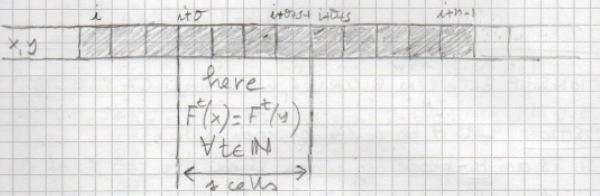
\includegraphics[width=.7\textwidth]{img/sistemi_complessi/parola_bloccante.png}
        \caption{Generalizzazione delle parole bloccanti che iniziano da $i$}
        \label{fig:parola_bloccante}
    \end{figure}
\end{nota}

\begin{nota}
    Se $u\in A^n$ è $s$-blocking allora ogni $v\in A^m$ con $m>n$ tale che ha 
    $u$ come sottosequenza allora anche $v$ è $s$-blocking.
\end{nota}

\begin{nota}
    Se $u\in A^n$ è $s_1$-blocking con un offset $\theta_1$ e $v\in A^m$ è  $s_2$-blocking
    con un offset $\theta_2$, allora $\forall w \in A^+$ la parola $uwv$ è una parola 
    bloccante. 
    La regione che va da $\theta_1$ a $s_2$ sarà lunga $n - \theta_1 + | w | + \theta_2 + s_2$.
\end{nota}

Le parole bloccanti sono in relazione con la stabilità degli automi cellulari.
\begin{teorema}
    Sia $F$ la regola globale per un CA di raggio $r$. Se $u$ è una parola $r$-bloccante
    allora l'insieme $\xi$ dei punti di equicontinuità di $F$ è infinito (e denso).
    \begin{proof}
        Sia $x\in A^\mathbb{Z}$ una qualsiasi configurazione del tipo $(uA^\ast)^+$,
        andremo a dismostrare che $x$ sia un punto di equicontinuità, ovvero 
        $$\forall n\in \mathbb{N} ,\exists m\in \mathbb{N} , \forall y\in A^\mathbb{Z}, y_{[-m,m]} = x_{[-m,m]} \implies \forall t\in \mathbb{N} F^t(y)_{[-n,n]}=F^t(x)_{[-n,n]}$$
        Scelto un $n \in \mathbb{N}$ e sua $m$ tale che $[-n,n]\subseteq [-m,m]$
        e $[-n,n]$ è contenuto all'interno del segmento $[-m,m]$ tale che 
        inizi all'interno segmento definito dal primo muro della prima occorrenza di $u$ in $[-m,m]$ fino 
        all'ultimo muro dell'ultima occorrenza di $u$. Allora $x$ è un punto di 
        equicontinuità. Questo deriva dal fatto che $u$ è $r$-bloccante, quindi un
        qualsiasi cambiamento esterno a $[-m,m]$ non influenza la regione interna
        delimitata dalla parola $u$.
    \end{proof} 
\end{teorema}
\begin{teorema}[\textbf{Caratterizzazzione della equiconinuità}]
    Sia $\langle A,r,f\rangle$ un CA e sia $F$ la regola globale allora i seguenti
    punti sono equivalenti:
    \begin{enumerate}
        \item \label{cond:non_carr_equi_1} $(A^\mathbb{Z}, F)$ è un \textbf{sistema equicontinuo}
        \item \label{cond:non_carr_equi_2} $\exists k>0$ tale che $\forall u \in A^{2k+1}$, $u$ è $r$-bloccante
        \item \label{cond:non_carr_equi_3} $(A^\mathbb{Z}, F)$ è \textbf{ultimamente periodico}
    \end{enumerate}
    \begin{proof}[dimostrazione opzionale]
        Dimostriamo le singole implicazioni:
        \begin{itemize}
            \item \ref{cond:non_carr_equi_1} $\implies $\ref{cond:non_carr_equi_2}:
            Sappiamo che il sistema è equicontinuo, quindi
            $$\forall n\in \mathbb{N} ,\exists k\in \mathbb{N} , \forall y,x\in A^\mathbb{Z}, y_{[-k,k]} = x_{[-k,k]} \implies \forall t\in \mathbb{N} F^t(y)_{[-n,n]}=F^t(x)_{[-n,n]}$$
            Sia $n=r$ allora 
            $$\exists k\in \mathbb{N} , \forall y,x\in A^\mathbb{Z}, y_{[-k,k]} = x_{[-k,k]} \implies \forall t\in \mathbb{N} F^t(y)_{[-r,r]}=F^t(x)_{[-r,r]}$$
            Pertanto sappiamo che esistono parole $r$-bloccanti e presa una qualsiasi $u\in A^{2k+1}$ è $(2k+1)$-bloccante se è anche $r$-bloccante.
            \item \ref{cond:non_carr_equi_2} $\implies $\ref{cond:non_carr_equi_3}: 
            andremo a mostrare che esistono $p>0$ e $q\ge 0$ tali che $F^{q+p} = F^q$.
            Per ogni $u\in A^{2k+1}$, consideriamo $x^{(u)}=^\infty u^\infty$ (per 
            definizione è spazialmentente periodica e per ipotesi $r$-bloccante).
            Sappiamo che $\{F^t(x^{(u)})_0\}_{t\in \mathbb{N}}$ è utilimamente periodica,
            allora  anche $\{F^t(x^{(u)})\}_{t\in \mathbb{N}}$ è ultimamente periodica.
            Questo significa che $\exists p_u>0$ e $q_u\ge 0$ tali che $F^{q_u+p_u}(x^{(u)})_0 =F^{q_u}(x^{(u)})_0 $.
            Sia $p=\text{mcd}\{p_u|u\in A^{2k+1}\}$ e $q=\max\{q_u|u\in A^{2k+1}\}$.
            Allora $\forall u\in A^{2k+1}, F^{q+p}(x^{(u)})_0 = F^{q}(x^{(u)})_0$.

            Sia $x\in A^\mathbb{Z}$ una qualsiasi configurazione e $u=x_{[-k,k]}$.
            Dal momento che $u$ è $r$-bloccante, $\forall t\in \mathbb{N}, F^t(x)$
             e $ F^t(x^{(u)})$ sono uguali per una finestra diu lunghezza $r$, 
             senza perdere d igeneralità supponiamo che contenga la cella $0$, allora 
             $F^{q+p}(x)_0 = F^{q}(x)_0$. Ora $\forall i\in \mathbb{Z}$
             $$F^{q+p}(x)_i = \sigma^i(F^{q+p}(x))_0 = F^{q+p}(\sigma^i(x))_0= F^{q}(\sigma^i(x))_0 = \sigma^i(F^{q}(x))_0 = F^{q}(x)_i$$

            \item \ref{cond:non_carr_equi_3} $\implies $\ref{cond:non_carr_equi_1}: 
            è già stata dimostrata.
        \end{itemize}
    \end{proof}
\end{teorema}
Se si negano le condizioni si ha la caratterizzazione per i sistemi sensibili
alle condizioni iniziali.

\begin{nota}
    Se il sistema è \textbf{equicontinuo} allora tutte le parole da un certo punto 
    in poi sono bloccanti, mentre se è \textbf{almeno equicontinuo} allora ne esisterà
    una che prima o poi diventerà bloccante.
\end{nota}

\begin{teorema}[\textbf{Caratterizzazzione dell\'almeno equiconinuità}]
    Sia $\langle A,r,f\rangle$ un CA e sia $F$ la regola globale allora i seguenti
    punti sono equivalenti:
    \begin{enumerate}
        \item \label{cond:non_carr_a_equi_1} $(A^\mathbb{Z}, F)$ non è \textbf{sistema 
        sensibile alle condizioni iniziali}
        \item \label{cond:non_carr_a_equi_2} $(A^\mathbb{Z}, F)$ ha una parola $r$-bloccante
        \item \label{cond:non_carr_a_equi_3} $(A^\mathbb{Z}, F)$ è \textbf{almeno equiconinuo}
    \end{enumerate}
    \begin{proof}
        Dimostriamo le singole implicazioni:
        \begin{itemize}
            \item \ref{cond:non_carr_equi_1} $\implies $\ref{cond:non_carr_equi_2}:
            per ipotesi il sistema non è sensibile alle condizioni iniziali quindi
            $$\forall n\in \mathbb{N} ,\exists x \in A^\mathbb{Z}, \exists m\in \mathbb{N} , \forall y\in A^\mathbb{Z}, y_{[-m,m]} = x_{[-m,m]} \land \forall t\in \mathbb{N} F^t(y)_{[-n,n]}\ne F^t(x)_{[-n,n]}$$
            Scegliamo arbitrariamente $n$ in modo tale che $2n+1\ge r$.
            $$\exists x \in A^\mathbb{Z}, \exists m\in \mathbb{N} , \forall y\in A^\mathbb{Z}, y_{[-m,m]} = x_{[-m,m]} \land \forall t\in \mathbb{N} F^t(y)_{[-n,n]}\ne F^t(x)_{[-n,n]}$$
            Quindi $u=x_{[-m,m]}$ è $(2n+1)$-bloccante quindi
            $$\forall z,z'\in A^\mathbb{Z}: z_{[-m,m]}=z'_{[-m,m]} = x_{[-m,m]} =u$$
            Questo significa che 
            $$\forall t, F^t(z)_{[-n,n]} = F^t(x)_{[-n,n]}\text{ e } F^t(z')_{[-n,n]} = F^t(x)_{[-n,n]}$$
            Quindi $F^t(z)_{[-n,n]} = F^t(z')_{[-n,n]},\forall t$. In conclusione $u$
            è anche $r$-bloccante da $2n+1\ge r$.
            \item \ref{cond:non_carr_equi_2} $\implies $\ref{cond:non_carr_equi_3}: 
            abbiamo già dimostrata.
            \item \ref{cond:non_carr_equi_3} $\implies $\ref{cond:non_carr_equi_1}: 
            se il sistema è A.E. allora esiste un punto di equicontinuità e quindi
            non può essere sensibile alle condizioni iniziali.
        \end{itemize}
    \end{proof}
\end{teorema}

\begin{teorema}
    Sia $\langle A,r,f\rangle$ un CA, è decidibile stabilire se data una word $u\in A^+$
    è $r$-bloccante
\end{teorema}

\begin{teorema}
    Il problema di stabilire se il CA ammette una parola $r$-bloccante 
    è indecidibile.
\end{teorema}

\begin{teorema}
    Stabilire se un CA è almeno equicontinuo o sensibile alle condizioni iniziali 
    è un problema indecidibile.
\end{teorema}

\begin{teorema}
    Stabilire se un CA è nilpotente è un problema indecidibile.
\end{teorema}

\begin{teorema}
    Stabilire se un CA è equicontinuo (o ultimamente periodico) è un problema indecidibile.
    \begin{proof} [cenni di dimostrazione]
        Per assurdo assumiamo che l'ultima periodicità è decidibile. Sia 
        $\langle A,r,f\rangle$  un CA e $F$ la sua regola globale, dal momento
        che l'ultima periodicità è decidibile, possiamo stabilire quando $F$ entra 
        nei seguenti casi:
        \begin{itemize}
            \item $F$ non è ultimamente periodica $\implies$ $F$ non è nilpotente
            \item $F$ è ultimamente periodica allora $\exists p>0, q\in \mathbb{N}$
            tale che $F^q=F^{q+p}$. Dalle configurazioni spazialmente periodiche,
            $p$ e $q$ sono computabili quindi:
            \begin{itemize}
                \item $p\ne 1\implies F$ non è nilpotente
                \item $p= 1$ allora:
                \begin{itemize}
                    \item Se $^\infty q^\infty$ è l'unica $x$ tale che $F(x)=x$ allora
                    $F$ è nilpotente
                    \item Altrimenti $F$ non è nilpotente
                \end{itemize}
            \end{itemize}
        \end{itemize}
    \end{proof}
\end{teorema}

\begin{definizione}[\textbf{Permutativa RM/LM}]
    $f:A^{2r+1}\rightarrow A$ è \textbf{permutativa} se 
    $$\forall b\in A, \forall u \in A^{2r}, \exists ! a\in A: f(ua)=b (f(au))=b$$
    Permutativa perché $\forall u \in A^{2r}, f_{|u}:A\rightarrow A:f_{|u}(a) = b$
    e $f_{|u}$ è biettiva.
\end{definizione}